%----------------------------------------------------------------------------
\chapter{Tervezés}
\label{chp:design}
%----------------------------------------------------------------------------
Ebben a fejezetben bemutatok egy olyan modellt, ami oktatási laborokat tud ábrázolni, illetve definiálok rajta végezhető terítési műveleteket, ezáltal magyarázva a terítési folyamat működését. Végül a fájlterítő alkalmazás felépítését részletezem.

\section{A labor modelljének tervezése}
\label{design_model}

Egy modell megalkotásakor érdemes először a feladatot könnyebben kezelhető részekre bontani, a mi esetünkben ez a modell három részre szedését eredményezi, ami \aref{fig:designmodelparts}-es ábra illusztrál. A három rész a laborban levő számítógépek (Computer), virtuális gépek (VirtualMachine) és a lehetséges terítési célállapotok (Lab).

\begin{figure}[ht]
	\centering
	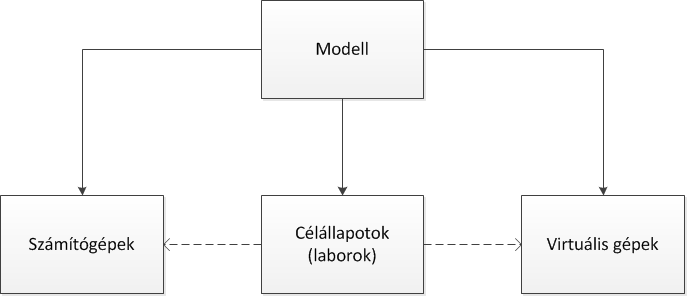
\includegraphics[width=100mm, keepaspectratio]{figures/design_modelparts.png}
	\caption{Labor modelljének három része.}
	\label{fig:designmodelparts}
\end{figure}

Vegyük először a virtuális gépek modelljét(\ref{fig:designvm}-es ábra)! A terítendő VM-ek azon tulajdonságainak kell a modellben megjelennie, amelyekre a fájlterítés során szükségünk lesz, ezek pedig a VM neve, őt tartalmazó fájl elérési útvonala és használatának követelményei. Utóbbinál a rendelkezésre álló memória mennyiségét, rendelkezésre álló szabad tárterület méretét és a rendszer architektúráját kell feltüntetnünk, mert csak ezek befolyásolják a gépekkel való kompatibilitást. Érdemes megkülönböztetni a Vagrant által készíttetendő VM-eket, mert róluk extra információkat kell eltárolnunk (VagrantVM a VirtualMachine leszármazottja lesz). Jobban átlátható modellt kapunk, ha a követelmények tárolását ``kiszervezzük'', és a Requirements osztályban tároljuk ahelyett, hogy minden VirtualMachine-nél attribútumként vennénk fel. Érdemes azt is eltárolnunk, hogy egy VM melyik számítógépen van, sok, a modellen értelmezhető művelet futási idejét tudjuk felgyorsítani vele, például ha egy adott VM-et szeretnénk majd törölni a gépekről, akkor nem kell az összesen végigmennünk, hanem közvetlen törölhetjük azokról, amelyiken rajta van.

\begin{figure}[ht]
	\centering
	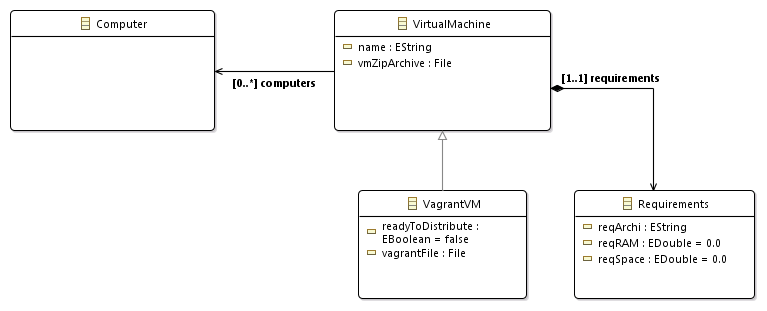
\includegraphics[width=130mm, keepaspectratio]{figures/design_vm.png}
	\caption{Labormodell - virtuális gépek}
	\label{fig:designvm}
\end{figure}

Hasonló megfontolásokkal készíthetjük el a számítógépek modelljét (\ref{fig:designcomputers}-as ábra), a számunkra fontos adatok itt a számítógép neve, elérhetősége és azon tulajdonságai, amik egy VM-el való kompatibilitást meghatároznak. Azt is el kell tárolnunk értelemszerűen, hogy adott számítógépen melyik virtuális gépek vannak már rajta. A számítógép elérhetőségeihez kapcsolódó attribútumokat nem csak azért tettük ConnectionInfo objektumokba, mint az előbbieknél a Requirements-be, hanem mert érzékeny adatokat is tárol (felhasználónév + jelszó).

\begin{figure}[ht]
	\centering
	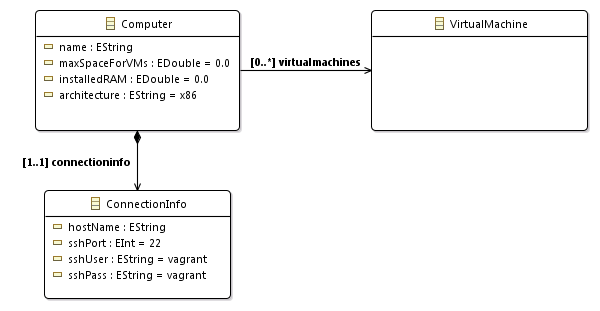
\includegraphics[width=110mm, keepaspectratio]{figures/design_computer.png}
	\caption{Labormodell - számítógépek}
	\label{fig:designcomputers}
\end{figure}

Az utolsó modellezendő dolog a terítés végállapota (\ref{fig:designlab}-es ábra), ami egy tanórához tartozó labor felépítését tartalmazza, vagyis az összes szükséges számítógép -> virtuális gép hozzárendelést. Ezt modell szinten úgy tudjuk leírni, hogy a végállapot tartalmaz minden számítógéphez egy ComputerConfig-ot, ami adott számítógépekre terítendő virtuális gépek listáját tartalmazza, és persze hivatkozik a konkrét számítógépre is.

\begin{figure}[h!]
	\centering
	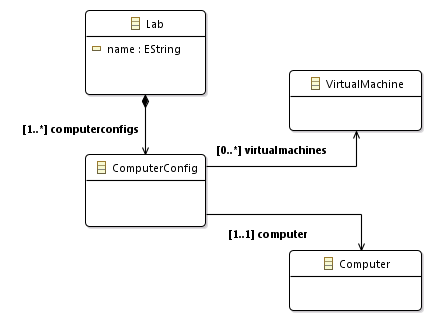
\includegraphics[width=100mm, keepaspectratio]{figures/design_lab.png}
	\caption{Labormodell - laborok(célállapotok)}
	\label{fig:designlab}
\end{figure}

Az előbb leírt modellrészletek összefogásához még szükségünk egy olyan elemre, ami mindhárom részt összefogja (\ref{fig:designmodelroot}-ös ábra). A LabSystem lesz a modell gyökéreleme, ez fogja tárolni a laborunkban található össze számítógépet, virtuális gépet és az összes felvett terítési végállapotot. Azt is itt tároljuk, hogy melyik számítógépet választjuk a Torrent alapú terítés során sedd-nek.

\begin{figure}[h!]
	\centering
	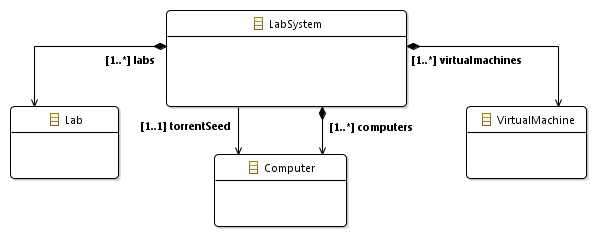
\includegraphics[width=130mm, keepaspectratio]{figures/design_modelroot.png}
	\caption{Labormodell - gyökérelem}
	\label{fig:designmodelroot}
\end{figure}

\section{Terítési műveletek a modellen}

Annak a megtervezésére, hogy egy fájlterítési folyamat hogyan zajlik érdemes azt kisebb darabokba vágni, azt definiálni egyszerű műveletekkel.
Az előbbi fejezetben ismertetett modellre definiálok itt terítési műveleteket, és megkísérlem leírni segítségükkel az egész fájlterítési folyamatot.
Az egyszerű műveleteket a következő formátumban fogom definiálni: MŰVELET\_NEVE(paraméter1\_neve: paraméter1\_típusa, paraméter2\_neve\ldots).

A modellen értelmezett terítési műveletek: [a többi modellen értelmezhető művelet, amitől teljes rendszerré válik a dolog, de a terítésnél nem relevánsak kellenek-e? Gondolok itt azokra, amik üres modellt hoznak létre, hozzáadnak pc-t/vm-et/lab-et az erőforrásokhoz.]

\begin{itemize}
  \item KÜLÖNBSÉG(cél: Lab, erőforrások: LabSystem): Ez a művelet a paraméterei között különbséget képez, vagyis a Lab-ből kiszedi azokat a (Computer, VirtualMachine) párokat, amik a LabSystem-ben már szerepelnek. Ennek az a célja, hogy a terítendő VM-ek közül kiszűrje azokat, amelyek már ott vannak, ahova terítenénk őket. Visszatérési érték: Lab, ami a duplikátumokat nem tartalmazza.
  \item TÖRÖL(törlendő\_vm : VirtualMachine, melyik\_gépekről: List<Computer>): Ezzel a művelettel törölhetjük a második paraméter Computer-eket tartalmazó lista összes eleméről az adott virtuális gépet. Visszatérési érték: nincs, a paraméterként kapott gépeknek módosítja a tartalmát.
  \item KOMPATIBILIS\_E(pc: Computer, vm: VirtualMachine): Arra a kérdésre válaszol, hogy adot VM kompatibilis-e a Computer-rel. Ellenőrzi az architektúrák megfelelését, a memória és a szabad lemezterület méretét. Visszatérési érték: IGAZ vagy HAMIS.
  \item FELTÖLT(vm: VirtualMachine, pc: Computer): Feltölti a VM-et a Computer-re, vagyis hozzáadja annak a \code{virtualmachines} listájához. Visszatérési érték: nincs, amennyiben már ott található a feltöltendő VM a PC-n, akkor a művelet nem csinál semmit.
\end{itemize}

Az előbbiek segítségével már felírható a TERÍTÉS(cél: Lab, erőforrások: LabSystem) művelet: [talán ábrával és nem pszeudokóddal?]

\code{TERÍTÉS(cél: Lab, erőforrások: LabSystem):}\\
\indent \code{duplikátumok\_nélküli\_cél = KÜLÖNBSÉG(cél, LabSystem)}\\
\indent \indent \code{FOR minden ComputerConfig a duplikátumok\_nélküli\_cél-ban}\\
\indent \indent \indent	\code{FOR minden VirtualMachine a ComputerConfig.Virtualmachines-ben}\\
\indent \indent \indent	\code{HA(KOMPATIBILIS(ComputerConfig.Computer, VirtualMachine))}\\
\indent \indent \indent \indent	\code{AKKOR FELTÖLT(VirtualMachine, ComputerConfig.Computer)}


\section{Fájlterítő alkalmazás architektúrája}
\label{design_apparchi}

\Aref{fig:designoverview}-os ábra fogja elmagyarázni az új terítési megoldás alapvető működési elvét: beolvassuk a modellt, ami alapján az egyik gépet seed-nek kiválasztva megcsináljuk a torrentes terítés. Az alkalmazás a terítésben szereplő gépektől (a torrent swarm-ja) futás közben a terítés állapotáról kér le információkat.

\begin{figure}[ht]
	\centering
	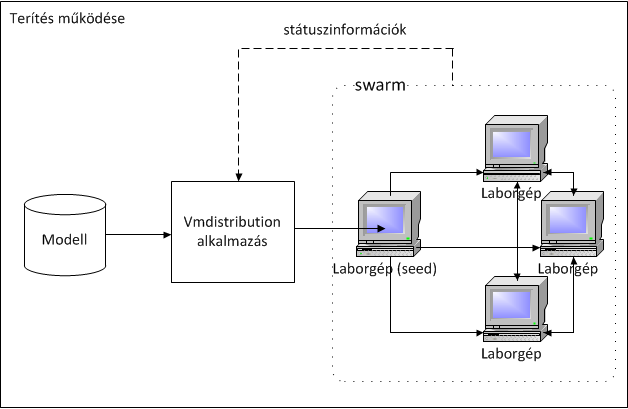
\includegraphics[width=130mm, keepaspectratio]{figures/design_overview.png}
	\caption{Új terítési megoldás működésének folyamata}
	\label{fig:designoverview}
\end{figure}

\Aref{fig:designprotocols}-es ábrán látjuk, hogy a terítés egyes szereplői hogyan és milyen protokollokat használva kommunikálnak egymással. [kell-e vajon ehhez, ill. az előzőhöz a tárhely, ahol a virtuális gépeket tároljuk?]

\begin{figure}[ht]
	\centering
	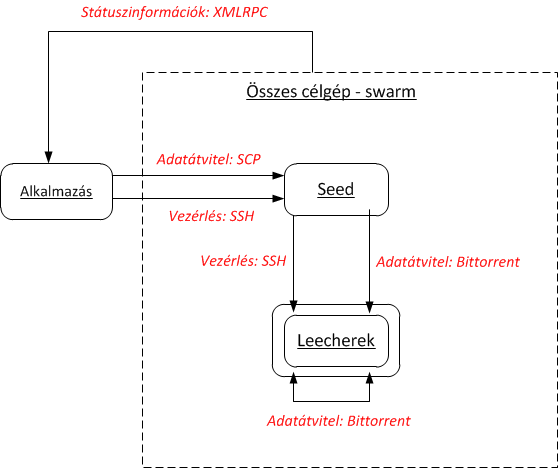
\includegraphics[width=140mm, keepaspectratio]{figures/design_protocols.png}
	\caption{Terítési folyamat egyes szereplői között használt kommunikációs protokollok}
	\label{fig:designprotocols}
\end{figure}

